\section{Input filter}
Input filtreret har som sådan ikke været en del af projektet, da det er blevet givet af Terma. Dette blev gjort, så der kunne fokuseres andetsteds. 

\noindent Herunder beskrives filtret dog stadig, så der gives forståelse for, hvordan det er designet og hvad det bruges til.

\noindent \cite{Inputfilter} Et input filter er nødvendigt i switch mode power supplies. For det første skal det sikre imod den elektromagnetiske interferens, der bliver genereret fra switching. Hvis denne interferens får lov at komme ud på forsyningsnetværket, vil det påvirke andet udstyr, hvilket selvfølgelig ikke er hensigtsmæssigt. Mængden af  tilladeligt EMI (elektromagnetisk interferens) er fastlagt af standarder verden over, så hvis ikke produktet overholder dette, kommer det aldrig på markedet.

\noindent Udover EMI skal filtret også sikre, at højfrekvent spænding fra forsyningsnettet, ikke når outputtet for power supplien. 

Det er i dette projekt gjort med et parallel dæmpet filter. Det består af et LC led, der giver en overordnet resonant frekvens. I sig selv, bør det kunne sikre sig imod de 2 punkter beskrevet ovenfor. Problemet i kun at bruge denne del, ligger ved knækfrekvensen. Når filtret er udæmpet, som det er ved et LC, kan der komme stor forstærkning ved cut off frekvensen, og derfor forstærke støjen ved den frekvens istedet. Det betyder at der gerne skal ligge en stor dæmpning ved frekvensen. Med en lille dæmpningsfaktor fås et stort gain ved cut off frekvensen og omvendt. En dårlig dæmpningsfaktor kan give resten af systemet en dårligere performance. Det kan gå ind og påvirke overføringsfunktionen til reguleringsloopet og på den måde få systemet til at oscillere. Hvis der sørges for, at udgangs impedans kurven for input filtret ligger meget under impedans kurven for konverteren, vil konverterens loop gain ikke blive ændret det store. Det vil sige, at det er vigtigt at holde peak impedancen nede for filtret, for at undgå oscillerings problemer forårsaget af inputfiltret.     

\noindent Det er her det parallelle led kommer ind i billedet. Det består af en modstand i serie med en kondensator. Meningen med modstanden er, at reducere udgangs peak impedancen af filtrets cutoff frekvens. Samtidig vil kondensatoren i serie med modstanden sørge for, at blokere DC delen af inputspændingen og derfor mindske effekttabet i modstanden. Denne kondensator skal have en mindre impedans end modstanden ved resonantfrekvensen og en større kapacitans end filter kapaciteten. Dette vil gøre, at cutoff frekvensen af R-L filtret ikke påvirkes af kondensatoren. På figur~\ref{fig: Inputfilter} ses hele filtret givet af Terma.    
\begin{figure}[H]
	\center
	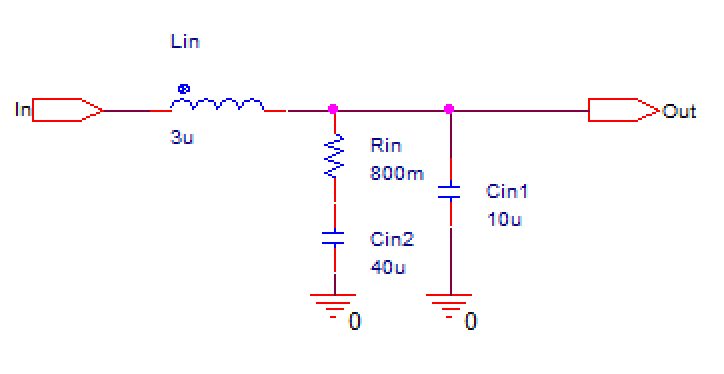
\includegraphics[max width=0.7\linewidth]{/tex/2iteration/billeder/Inputfilter.png}
	\caption{Inputfilter}
	\label{fig: Inputfilter}
\end{figure}
Det ses, at filtret har en overordnet knækfrekvens på:
\begin{equation} \label{fc}
f_c = \frac{1}{2 \cdot \pi \cdot \sqrt{3\micro H \cdot 10\micro F}} = 29.06kHz
\end{equation}
Samtidig kan det konkluderes, at selve kapaciteten på $C_{in2}$ er 4 gange større end $C_{in}$ samt impedansen bliver:
\begin{equation} \label{XC2}
X_{Cin2} = \frac{1}{2 \cdot \pi \cdot 40\micro F \cdot 29.06kHz} = 0.137\ohm
\end{equation}
Hvilket er mindre end modstanden på $0.8\ohm$. Det vil sige, at filtret opfylder kriterier opstillet ovenfor.